\section{Preliminaries}
\subsection{Event Structure}
\begin{definition}[Event Structure]
    An event structure is a triple $\mr{E} = (E,\#,\vdash)$ where:
    \begin{enumerate}
        \item $E$ is a set of events
        \item \# is a binary symmetric, irreflexive relation on $E$,
              the conflict relation.
              We shall write $Con$ for the set of 
              \textit{consistent} subsets of $E$,
              i.e. those finite subsets $X \subseteq E$ for which:
              $\forall e,e' \in X . \neg (e\#e')$
        \item $\vdash \subseteq Con \times E$ is the enabling relation which satisfies:
              $ X \vdash e \ \wedge \ X \subseteq Y \in Con \Rightarrow Y \vdash e$
    \end{enumerate}

\end{definition}

\begin{comment}
    salam
\end{comment}

\begin{notion}{$(\doublevee)$}
    In an event structure we shall write $\doublevee$ for the reflexive conflict relation by which we mean
    that $e\doublevee e'$ in an event structure iff either $e\#e'$ or $e=e'$.
\end{notion}

\begin{notion}{$(\vdash_{min})$}
    For any event structure we can define the minimal enabling relation $\vdash_{min}$ by:
    \begin{align*}
        X \vdash_{min} e \iff X \vdash e \wedge
        ( \forall Y \subseteq X . Y \vdash e \Rightarrow Y = X )
    \end{align*}
\end{notion}

\begin{definition}[Configuration]
    \label{conf}
    Let $\mr{E} = (E,\#,\vdash)$ be an event structure.
    Define a \textit{configuration} of $\mr{E}$ to be a subset of events $x \subseteq E$ which is
    \begin{enumerate}
        \item consistent: $x \in Con$
        \item secured: $\forall e \in x. \exists e_0,...,e_n \in x. e_n = e \ \wedge
                  \forall i \leq n. \s{e_0,...,e_{i-1}} \vdash e_i$
    \end{enumerate}
\end{definition}
\noindent The set of all configurations of an event structure is written as $\mathcal{F}(E)$.
It is helpful to unwrap condition (2) a little. It says an event $e$ is secured in a set $x$
iff there is a sequence of events $e_0,...,e_n = e$ in $x$ such that:
\begin{align*}
    \emptyset \vdash e_0, \s{e_0} \vdash e_1, ..., \s{e_0,...,e_{i-1}} \vdash e_i,...,
    \s{e_0,...,e_{n-1}} \vdash e_n.
\end{align*}
We call such a sequence $e_0,e_1,...,e_n = e$ a \emph{securing} for $e$ in $x$.

\begin{definition}[Labelled Event Strtucture]
    A labelled event structure consists of $(E,\#,\vdash,L,l)$ where
    $(E,\#,\vdash)$ is an event structure, $L$ is a set of labels,
    not including the element *, and $l$ is a function $l: E \rightarrow L$
    from its events to its labels.
\end{definition}
\begin{example}
    Here we define an event structure for capturing the 
    behavior of the example \ref{example:loop}.
    To do so, first we encode the network using a language for SDNs and 
    then we use event structure as a semantic model of the language 
    and derive the event structure.
    Since the SDN language and its event structure semantic
    is out of the scope of this paper, here we only describe the 
    resulting event structure.
    Let $\mr{E} = (E,\vdash, \#)$ be the event structure of the network update.
    We define events $p,q$ for the updates and an event $bb$ that denotes
    the forwarding of packet from $b$ to $b$ which indicates a loop in the 
    network.
    For simplicity, we omit all other events from event structure such as 
    forwarding from $a$ to $d$.
    Thus we consider $E = \s{p,q,bb}$.
    The update $p$ allows $bb$ to happen, thus capture this behavior with 
    $p \vdash_{min} bb$.
    If both $p$ and $q$ happened in the network then $bb$ can not happen.
    So, we add a conflict between $q$ and $bb$.
    Furthermore, note that $p$ and $q$ can be done unconditionally, thus 
    we have $\e \vdash p$ and $\e \vdash q$.
    Figure \ref{fig:loop:es} shows the configuration lattice of this 
    event structure.
    We can see that $\s{p,bb}$ is an unsafe configuration of this event structure. 

    \begin{figure}
        \centering
        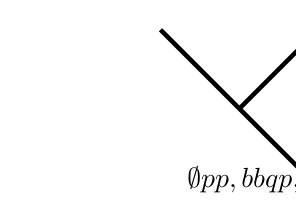
\begin{tikzpicture}
            \crd{0}{0}{$\emptyset$}
            \crd[left]{-1}{1}{$\s{p}$}
            \crd[left]{-2}{2}{$\s{p,bb}$}
            \crd[right]{1}{1}{$\s{q}$}
            \crd[right]{0}{2}{$\s{p,q}$}
            \draw [ultra thick] (0,0) -- (1,1);
            \draw [ultra thick] (0,0) -- (-1,1);
            \draw [ultra thick] (-1,1) -- (0,2);
            \draw [ultra thick] (1,1) -- (0,2);
            \draw [ultra thick] (-1,1) -- (-2,2);
        \end{tikzpicture}
        \caption{Lattice of configurations}
        \label{fig:loop:es}
    \end{figure}
\end{example}

\subsection{Causal Model \cite{hp}}
A signature $\mathcal{S}$ is a tuple $(\mathcal{U},\mathcal{V},\mathcal{R})$,
where $\mathcal{U}$ is a set of exogenous variables, $\mathcal{V}$
is a set of endogenous variables, and $R$ associates with every variable
$Y\in \mathcal{U}\cup \mathcal{V}$ a nonempty set $\mathcal{R}(Y)$ of possible values for $Y$.
A causal model (or structural model) over signature $S$ is a tuple
$M=(\mathcal{S},\mathcal{F})$, where $\mathcal{F}$ associates with
each variable $X \in \mathcal{V}$ a function denoted $F_X$ such that
$F_X: (\times_{U\in \mathcal{U}}\mathcal{R}(U))\times (\times_{Y\in\mathcal{V}-\{X\}}\mathcal{R}(Y))\rightarrow \mathcal{R}(X)$.

$F_X$ determines the value of $X$ given the values of all the other variables
in $\mathcal{U}\cup \mathcal{V}$.
For example, if $F_X(Y,Z,U)=Y+U$ (which we usually write as $X = Y + U$),
then if $Y=3$ and $U=2$, then $X = 5$, regardless of how $Z$ is set.
These equations can be thought of as representing processes (or mechanisms) by which values are assigned to variables. Hence, like physical laws, they support a counterfactual interpretation.
For example, the equation above claims that in the context $U=u$, if $Y$ were 4, then $X$ would be $u+4$ (which we write as $(M,u) \models [Y\leftarrow 4](X = u + 4))$, regardless of what values X, Y, and Z actually take in the real world.


The function $\mathcal{F}$ defines a set of (\textit{modifiable}) \textit{structural equations} relating to the values of the variables.

\subsubsection{Causal Network}
We can describe a causal model $\m$ using a causal network.
This is a graph with nodes corresponding to the random variables
in $\mathcal{V}$ and an edge from a node labeled $X$ to one
labeled $Y$ if $F_Y$ depends on the value of $X$.
This graph is a dag that follows from the assumption that the
equations are recursive.
We occasionally omit the exogenous variables $\vec U$ from the causal network.

\subsubsection{Actual Cause}
Given a signature $S= (\mathcal{U},\mathcal{V},\mathcal{R})$, a formula of the form $X =x$, for $X \in \mathcal{V}$ and $x \in \mathcal{R}(X)$, is called a \textit{primitive event}.
A \textit{basic causal formula} is one of the form $[Y_1 \leftarrow y_, ..., Y_l\leftarrow y_k]\varphi$, where $\varphi$ is a Boolean combination of primitive events, $Y_1,...,Y_k$ are distinct variables in $\mathcal{V}$, and $y_i \in \mathcal{R}(Y_i)$.
Such a formula is abbreviated as $[\vec{Y}\leftarrow\vec{y}]\varphi$.
A \textit{causal formula} is a Boolean combination of basic causal formulas.
A causal formula $\psi$ is true or false in a causal model, given a context.
We write $(M,\vec u)\models \psi$ if $\psi$ is true in causal model $M$ given context $\vec u$.
$(M,\vec u)\models [\vec Y\leftarrow \vec y](X=x)$ if the variable $X$ has value $x$ in the unique solution to the equation in $M_{\vec{Y} \leftarrow \vec{y}}$ in context $\vec u$.
The context and structural equations are given.
They encode the background knowledge.
All relevant events are known.
The only question is picking out which of them are the cause of $\varphi$ or, alternatively, testing whether a given set of events can be considered the cause of $\varphi$.
The types of events that we allow as actual causes are ones of the form $X_1 = x_1 \wedge ... \wedge X_k=x_k$-- that is, conjunctions of primitives events.
We abbreviate this as $\vec X = \vec x$.
\begin{definition}[Actual Cause]
    $\vec X = \vec x$ is an actual cause of $\varphi$ in $(M,\vec u)$ if the following three conditions hold:
    \begin{itemize}
        \item  \textbf{AC1.} $(M,\vec u)\models (\vec X = \vec x) \wedge \varphi$.
              (both $\vec X = \vec x$ and $\varphi$ are true in actual world)
        \item  \textbf{AC2. }There exists a partition $(\vec Z, \vec W)$ of $\mathcal{V}$ with $\vec X \subseteq \vec Z$ and some setting $(\vec x',\vec w')$ of the variables in $(\vec X,\vec W)$ such that if $(M,\vec u)\models \vec Z = z^*$ for all $Z\in \vec Z$, then both of the following conditions hold:

              (a) $(M,\vec u)\models[\vec X \leftarrow \vec x', \vec W \leftarrow \vec w']\neg \varphi$.

              (b) $(M,\vec u)\models[\vec X\leftarrow \vec x, \vec W \leftarrow \vec w']\varphi$ .

              (c) $(M,\vec u)\models[\vec X\leftarrow \vec x, \vec W \leftarrow \vec w', \vec Z'\leftarrow \vec z^*]\varphi$ for all subsets $Z'$ of $\vec Z$.

        \item  \textbf{AC3.} $\vec X$ is minimal; no subset of $\vec X$ satisfies conditions $AC1$ and $AC2$.
    \end{itemize}
\end{definition}
We call the tuple $(\vec W, \vec w,\vec x')$ a witness to the fact that $\vec X=\vec x$ is a cause of $\varphi$.

\begin{definition}[But-For Cause]
    We say $\vec X = \vec x$ is a but-for cause of $\varphi$ in
    $(M,\vec u)$ if there exists a witness $(\vec W, \vec w, \vec x')$
    for $\vec X = \vec x$ being an actual cause of $\varphi$
    where $\vec W = \emptyset $.
\end{definition}

Note that, if we consider a witness $(\vec W, \vec w, \vec x')$
for checking whether $\vec X = \vec x$ is a cause of $\varphi$
in $(M,\vec u)$ where $\vec W = \e$, then in the AC2(b) condition
we only need to check whether $(M,\vec u) \vDash [\vec X \leftarrow \vec x, \vec Z' \leftarrow \vec z^*]\varphi$ for all subsets $\vec Z'$
of $\vec Z$.
Since we have $(M,\vec u) \vDash (\vec X = \vec x)$ and
$(M,\vec u) \vDash Z = z^*$ for all $Z \in \vec Z$,
the Interventions $\vec X \leftarrow \vec x$ and
$\vec Z ' \leftarrow \vec z^*$ actually do not change the value of
any variable thus checking whether
$(M,\vec u) \vDash [\vec X \leftarrow \vec x, \vec Z' \leftarrow \vec z^*]\varphi$ is true
reduces to check whether $(M,\vec u) \vDash \varphi$
which must be already satisfied when we have checked AC1 condition.
This means that, to check whether $\vec X = \vec x$ is an actual cuase when using a witness with an empty $\vec W$
we only need to check AC1 and AC2(a) conditions.
\subsection{Extended Causal Model}
An extended causal model is a tuple $(\mathcal{S},\mathcal{F},
    \mathcal{E})$, where $(\mathcal{S},\mathcal{F})$ is a causal model, and $\mathcal{E}$ is a set of allowable settings for the endogenous variables.
That is, if the endogenous variables are $X_1,...,X_n$ then
$(x_1,...,x_n) \in \mathcal{E}$ if $X_1 = x_1, ..., X_n=x_n$ is an
allowable setting.
We say that a setting of a subset of the endogenous variables is allowable if it can be extended to a setting in $\mathcal{E}$.